\documentclass{article}
\usepackage{amssymb,amsmath}
\usepackage{graphicx}
\graphicspath{{./photos/}}
\title{Seven Sketches in Compositionality – Exercises}
\author{Adam Catto}
\date{}
\begin{document}
\maketitle
\section{Chapter 1 –– Generative Effects: Orders and Galois Connections}
\textbf{(1.1)}
\begin{itemize}
\item[(a)] 
\textit{order-preserving}  $f: x\mapsto x+1$\\
\textit{non-order-preserving}  $f: x\mapsto -x$
\item[(b)] \textit{metric-preserving} $x\mapsto x+2$\\
\textit{non-metric-preserving} $x\mapsto 2x$
\item[(c)] \textit{addition-preserving} $x\mapsto x$\\
\textit{non-addition-preserving} $x\mapsto 2x$
\end{itemize}\bigskip
\textbf{(1.2)}\\
 \\
 Circle 21, Circle the rest, box around the whole thing. i.e.
 $$\{ \{ 21 \}, \{ 11,12,13,22,23 \} \}$$\bigskip
\textbf{(1.6)}
\begin{enumerate}
	\item True
	\item False
	\item True
\end{enumerate}\bigskip
\textbf{(1.7)}
\begin{enumerate}
	\item $\{ \}, \{ 1\}, \{ 2\}, \{ 3\}, \{ 1,2\}, \{1,3\}, \{ 2,3\}, \{ 1,2,3\}$
	\item $\{ 1\} \cup \{ 1,3\} = \{ 1,3\}$
	\item $(h,1),(h,2),(h,3),(1,1),(1,2),(1,3)$
	\item $(h,1),(1,1),(1,2),(2,2),(3,2)$
	\item $A\cup B = \{ h,1,2,3\}$
\end{enumerate}\bigskip
\textbf{1.11}
\begin{enumerate}
	\item If there were more than one $p'\in P'$ such that $A_p=A'_{p'}$ (i.e. $p'_1$ and $p'_2$ such that $A_p=A'_{p'_1}$ and $A_p=A'_{p'_2}$), then $p'_1\neq p'_2$, so necessarily $A'_{p'_1} \cap A'_{p'_2}=\emptyset$. But then since $A'_{p'_1}=A_p=A'_{p'_2}$, then $A'_{p'_1}=A'_{p'_2}$, thus $A'_{p'_1}\cap A'_{p'_2} = A_p\cap A_p = A_p\neq \emptyset$, by definition of partition, therefore there cannot be more than one $p'\in P'$ such that $A_p=A'_{p'}$. $\hfill \blacksquare$
	\item Since there exists a $p'\in P'$ such that $A_p=A'_{p'}$, and by 1.11.1, there is at most one such $p'$, it follows that there is a bijection between these $p\in P$ and $p'\in P'$, thus $\forall p'\in P'$ there exists a $p\in P$ such that $A_p=A'_{p'}$. $\hfill \blacksquare$
\end{enumerate}\bigskip
\textbf{1.12}
$$ (11,11),(12,12),(13,13),(21,21),(22,22),(23,23),(11,12),(12,11),(22,23),(23,22) $$
\textbf{1.15}
\begin{enumerate}
	\item Each $A_p$ is $(\sim )$-connected, therefore they are nonempty.$\hfill\blacksquare$
	\item If $A_p\cap A_q\neq\emptyset$, then for any $x\in A_p\cap A_q$, it follows  that $x\in A_p$ and $x\in A_q$. Thus for any $x_p\in A_p$, we have $x_p\sim x$, and under $(\sim )$-closure and $x\in A_q$, it follows that $x_p\in A_q$, and the same for $x_q\in A_q$. Therefore, $A_p=A_q \vDash p=q$, which violates the contextual assertion that $p\neq q$, therefore $p\neq q\implies A_p\cap A_q=\emptyset$.$\hfill\blacksquare$
	\item Each $A_p$ is nonempty and $\sim$ is reflexive, i.e. we have at least for each $x$ that $x\sim x$, therefore we have at least that $A$ is the union of singleton sets that cover $A$, therefore $A=\bigcup_{p\in P} A_p$.$\hfill\blacksquare$
\end{enumerate}\bigskip
\textbf{1.19}
\begin{enumerate}
	\item $f:\mathbb{Z}\rightarrow\mathbb{R}: x\mapsto x+1$
	\item $f:\mathbb{Q}\rightarrow\mathbb{Z}: x\mapsto x-\frac{x}{10}$
	\item (1): yes (2): no (3): no (4): yes 
	\item (1): neither (2): top dot's targets are not unique, bottom dot has no target (3): top dot has no target (partial function?) (4) bijective
\end{enumerate}\bigskip
\textbf{1.20}\\
 \\
By function definition, each $a\in A$ has a unique $y\in\emptyset$ such that $(a,y)\in f$. But there are no $y\in\emptyset$, therefore there cannot exist any such $a\in A$, therefore $A$ is empty.$\hfill\blacksquare$\\
 \\
\textbf{1.33}\\
 \\
$
\begin{vmatrix}
a & 1 & 2\\
b & 1 & 3\\
c & 1 & 3\\
d & 2 & 2\\
e & 2 & 3
\end{vmatrix}
$\\
 \\
\textbf{1.35}\\
 \\
$(1,1),(1,2),(1,3),(2,2),(2,3),(3,3),(4,4)$\\
 \\
\textbf{1.41}\\
 \\
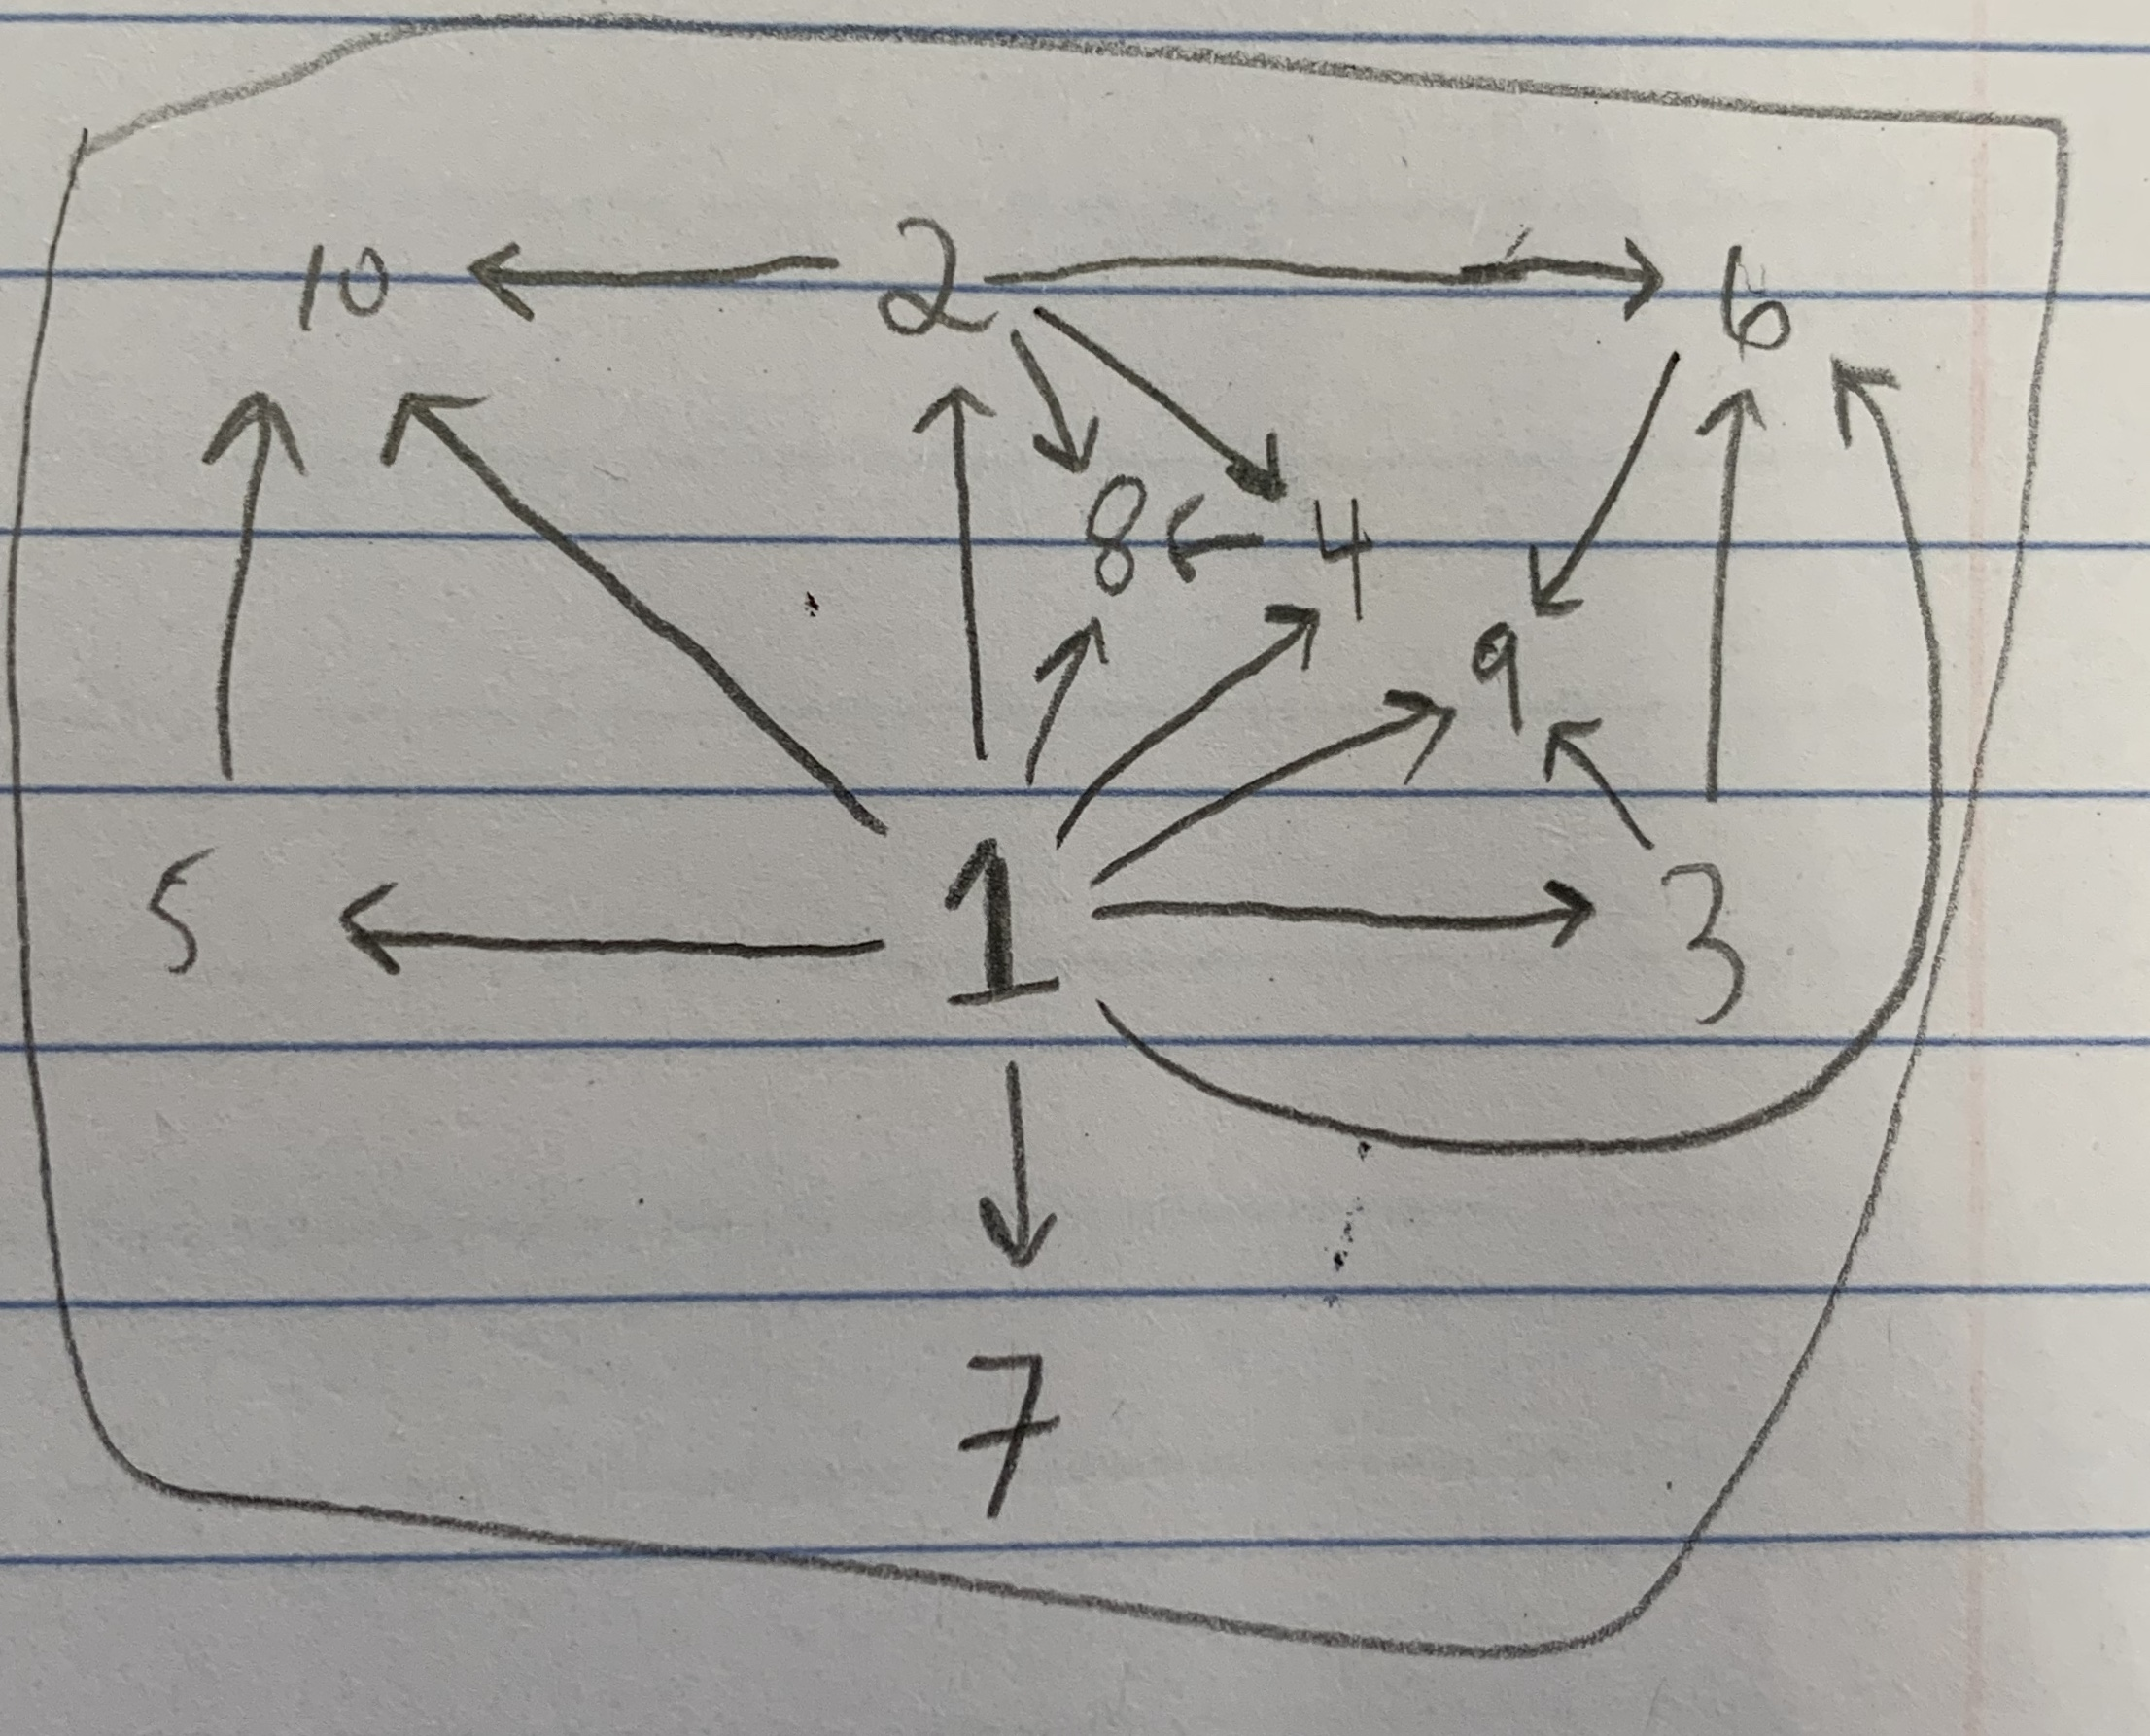
\includegraphics[scale=0.1]{7sketches-1-41.jpg}\\
It is not a total order; for instance, neither $7\leq 9$ nor $9\leq 7$.\\
 \\
\textbf{1.43}\\
 \\
Yes.\\
 \\
\textbf{1.46}\\
 \\
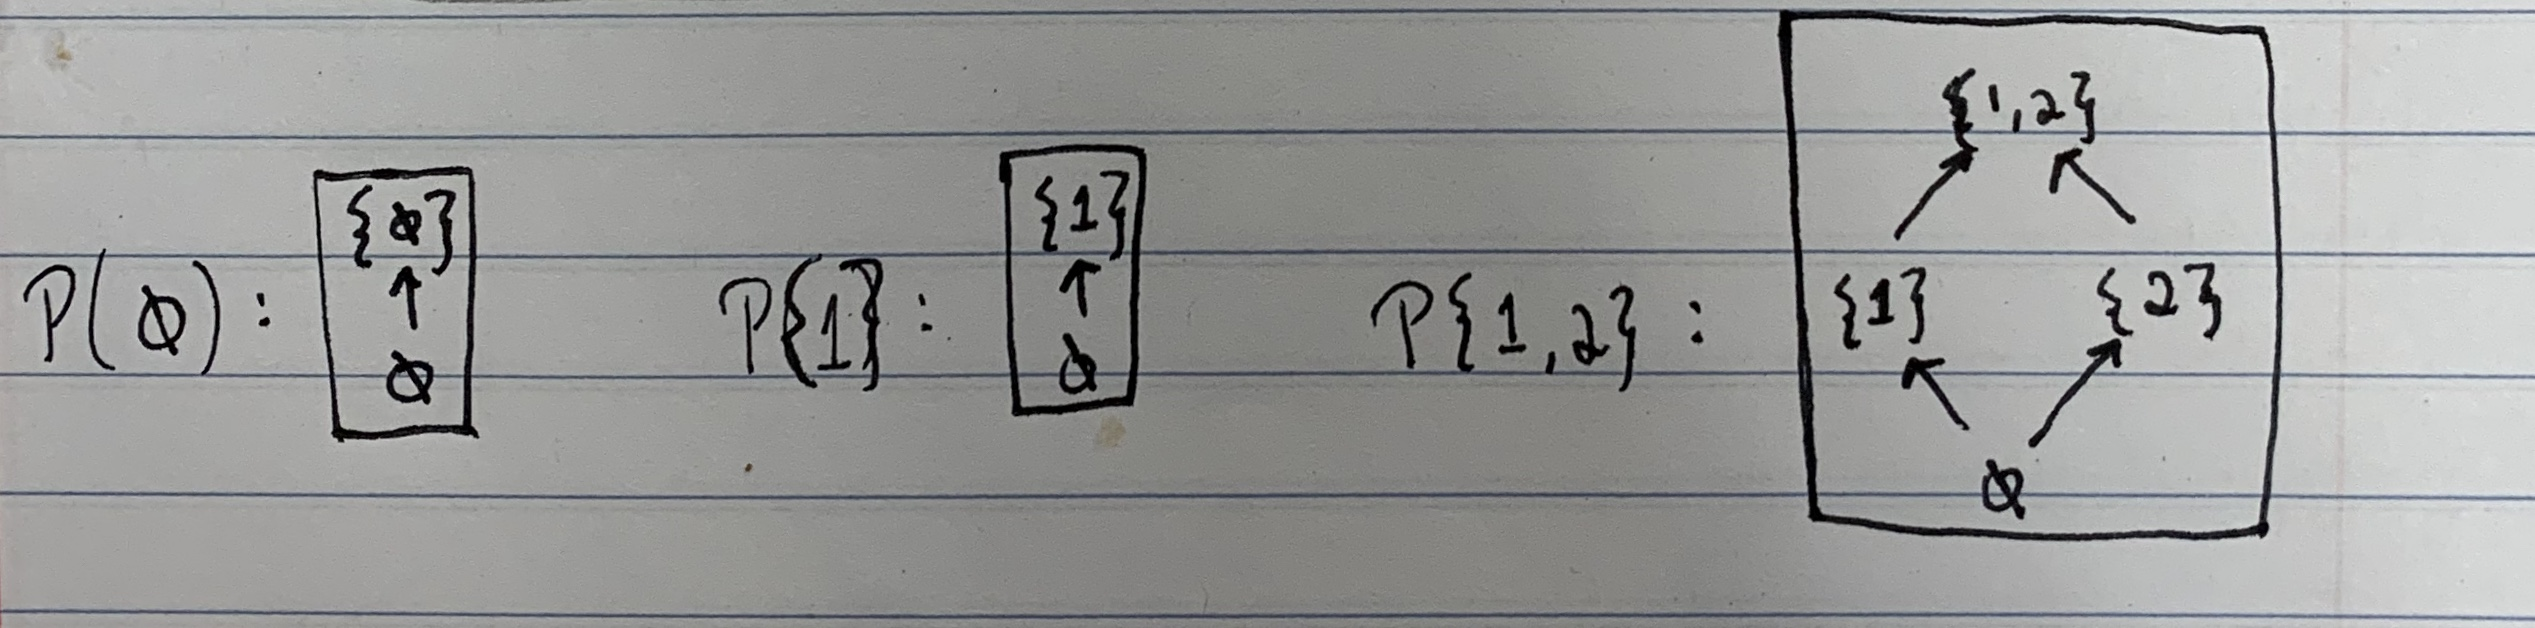
\includegraphics[scale=0.1]{7sketches-1-46.jpg}
\newpage
\textbf{1.48}\\
 \\
\textit{Coarsest}: identity function (top level of Hasse diagram) \\
\textit{Finest}: projection onto singleton sets for each $s\in S$ (second to bottom level of Hasse diagram)\\
 \\
\textbf{1.50}\\
 \\
This is the same as proving that all subsets of $X$ are upper sets of the discrete preorder on $X$, i.e. that $\forall \left[x,y\in X\right].\left[ x\in U \wedge x\leq y \implies y\in U \right]$. The empty set is in $U$ via vacuous truth of the antecedent. Also, each $\{ x\}$ for $x\in X$ is an upper set, via reflexivity of (discrete) preorder. Then for any $x\in X$, take the union of the singleton set $\{ x \}$ and any other subset $Y\subseteq X$ disjoint from this singleton. By the argument from two sentences ago, each such singleton set is an upper set. This union is a subset of $X$, and furthermore it is an upper set, since the antecedent conjunction is false – it is not the case that $x\leq y$ for any $y\in Y$, since they are not comparable via definition of discrete preorder. Therefore all such $Y$ are upper sets. These three statements (empty set is an upper set, all singletons are upper sets, all other subsets are upper sets) entail that all subsets of $X$ are upper sets, therefore the preorder of upper sets on $X$ is the power set.$\hfill\blacksquare$\\
 \\
 \textbf{1.61} \ \ \ \ \textit{(Yoneda Lemma for Preorders)}
 \begin{enumerate}
 	\item We have $p\in \uparrow p$ via reflexivity of $\leq$, and exactly when $p\leq p'$ we have $p'\in\uparrow p$; this is exactly the definition of upper set.$\hfill\blacksquare$
 	\item For $x,y\in P$, if $x\leq y$ then $x\leq^{OP} y$ in $P^{OP}$. There's an obvious map $\uparrow$ from $P^{OP}$ to the set of upper sets of elements of $P$, $U(P)$ as defined in (1.61.1). $U(P)$ is preordered via the subset relation. Recalling that $x\leq^{OP} y\iff y\leq x$, then we must show that $x\leq^{OP}y \implies \uparrow (x)\subseteq \uparrow (y)$, i.e. $y\leq x\implies \uparrow (x)\subseteq \uparrow (y)$. $y\leq x$, and due to transitivity of $\leq$, if $x\leq z$, then $y\leq z$, i.e. if $z\in\uparrow (x)$ then $z\in\uparrow (y)$, thus $\uparrow (x)\subseteq \uparrow (y).\hfill\blacksquare$
 	\item Suppose $p\leq p'$ in $P$. Then $p'\leq^{op} p$, and due to monotonicity of $\uparrow$ on the domain $P^{op}$, $\uparrow (p')\subseteq \uparrow (p)$.\\
 	Now suppose that $\uparrow (p')\subseteq \uparrow (p)$. Then for every element $x\in P$ such that $x\leq p$, it follows that $x\leq p'$. Then there exists a $y\in P$ such that $p\leq y\leq p'$, therefore $p\leq p'$.$\hfill\blacksquare$
 \end{enumerate}\bigskip
\textbf{1.66}\bigskip
\begin{enumerate}
	\item $x\leq y\implies id(x)\leq id(y)\implies x\leq y$
	\item for $p_1,p_2\in P$, $p_1\leq p_2 \implies f(p_1)\leq f(p_2)$, and for $q_1,q_2\in Q$, $q_1\leq q_2 \implies g(q_1)\leq g(q_2)$. Let $q_1=f(p_1), \ q_2=f(p_2)$. Then $p_1\leq p_2\implies g(f(p_1))\leq g(f(p_2))$, i.e. $(f;g)$ is monotone.$\hfill\blacksquare$
\end{enumerate}\bigskip
\textbf{1.80}
\begin{enumerate}
	\item Check that $p$ is $\leq$ each element: $p\leq p$; and that each least element is $\leq$ to $p$: $p\leq p \implies p\leq p.\hfill\blacksquare$
	\item If $P$ is a partial order, then if $x\equiv y\iff x=y$. It follows that if $\bigwedge A\equiv p$, then $\bigwedge A=p.\hfill\blacksquare$
	\item Yes, these are still true if we replace meets with joins. This can be checked simply by replacing $\leq$ with $\leq^{op}$, and that $p\leq^{op} p$ entails $p\leq p$.$\hfill\blacksquare$
\end{enumerate}\bigskip
\textbf{1.92}\\
 \\
A right adjoint for $(3\times –)$ is $\lfloor –/3 \rfloor$. We check that $x\leq \lfloor y/3\rfloor\iff 3x\leq y$. \\
$\left(\Rightarrow\right)$ Suppose $x\leq\lfloor y/3\rfloor$. Since $\lfloor y/3\rfloor\leq y/3$, it follows that $x\leq y/3$, thus $3x\leq y$.\\
$\left(\Leftarrow\right)$ Suppose now that $3x\leq y$. Then $x\leq y/3 \implies \lfloor x\rfloor\leq \lfloor y/3\rfloor$, and since $x\in\mathbb{Z}$, it follows that $\lfloor x\rfloor=x$, therefore $x\leq\lfloor y/3\rfloor .\hfill\blacksquare$\\
 \\
\textbf{1.93}
\begin{enumerate}
	\item $f(1)=1\implies 
\begin{vmatrix} \ \ 
	1\leq 1\implies g(1)=2\implies 1\leq 2\\
	1\leq 2\implies g(2)=2\implies 1\leq 2\\
	1\leq 3\implies g(3)=3\implies 1\leq 3
\end{vmatrix}\\
 \\
f(2)=1\implies \ \ 
\begin{vmatrix}
	1\leq 1\implies g(1)=2\implies 2\leq 2\\
	1\leq 2\implies g(2)=2\implies 2\leq 2\\
	1\leq 3\implies g(3)=3\implies 2\leq 3
\end{vmatrix}\\
f(3)=3\implies \left[ 3\leq 3\implies g(3)=3\implies 3\leq 3\right]
$\\
 \\
therefore $f$ is left-adjoint to $g.\hfill\blacksquare$
\item $f(1)=1\implies 
\begin{vmatrix} \ \ 
	1\leq 1\implies g(1)=2\implies 1\leq 2\\
	1\leq 2\implies g(2)=2\implies 1\leq 2\\
	1\leq 3\implies g(3)=3\implies 1\leq 3
\end{vmatrix}\\
 \\
f(2)=2\implies \ \ 
\begin{vmatrix}
	2\leq 2\implies g(2)=2\implies 2\leq 2\\
	2\leq 3\implies g(3)=3\implies 3\leq 3
\end{vmatrix}\\
 \\
f(3)=3\implies \left[ 3\leq 3\implies g(3)=3\implies 3\leq 3\right]
$\\
 \\
therefore $f$ is left-adjoint to $g.\hfill\blacksquare$
\end{enumerate}
 \newpage
\section{Chapter 2 – Resource Theories: Monoidal Preorders and Enrichment}
\textbf{(2.4)}\\
 \\
This fails due to condition \textit{(a)} of Definition (2.1) –\\ 
$\forall \left[ x_1,x_2,y_1,y_2 \in X\right] .\left[ (x_1\leq y_1 \wedge x_2\leq y_2)\implies x_1\otimes x_2 \leq y_1 \otimes y_2 \right] $\\
for instance, any model in which $x_1,x_2$ are both negative real numbers larger in magnitude than positive reals $y_1,y_2$ will not yield $x_1\otimes x_2 \leq y_1\otimes y_2.\hfill\blacksquare$\\
 \\
\textbf{(2.6)}\\
 \\
Yes, \textbf{Disc}$_M$ is indeed a symmetric monoidal preorder. It satisfies conditions (b) and (c) of Definition (2.1) via equation (2.2). It satisfies condition (d) of Definition (2.1) via the asserted commutativity of $*$. Finally, this induces satsifaction of condition (a) of Definition (2.1), via renaming of identical variables: if $m=n$ and $s=t$, then $m*s=n*s=n*t.\hfill\blacksquare$
\end{document}